\documentclass[a4paper,article]{article}

% Шрифты
\usepackage{fontspec}
\usepackage[14pt]{extsizes}
\setmainfont{Times New Roman}

% Языки
% Русский обязательно идёт вторым. Иначе не работают переносы
\usepackage[english, russian]{babel}

% Параметры страницы
\usepackage[left=3cm, top=2cm, right=1.5cm, bottom=2cm]{geometry}
\usepackage[onehalfspacing]{setspace}

% Параметры текста
% По умолчанию LaTeX не делает отступ после \section. Вроде как оно и не надо, но в тексте ВКР пусть лучше будет. В требованиях отступ описан. Этот пакет своим наличием добавляет этот отступ
\usepackage{indentfirst}
% По умолчанию абзацный отстум меньше требуемого. Задаём конкретный
\setlength{\parindent}{1.25cm}

% Цвета
\usepackage{xcolor}
\definecolor{cc-default}{rgb}{0.00, 0.00, 0.00}
\definecolor{cc-url}{rgb}{0.42, 0.60, 0.73}
% Задание основного цвета текста
\color{cc-default}
% Цвет вокруг текста
\usepackage{soul}
\sethlcolor{cc-accent-auxiliary}
\usepackage[colorlinks, allcolors=cc-default]{hyperref}
\urlstyle{rm}

% Пункты оглавления
\usepackage{titlesec}
\titleformat{\section}
{\centering\normalfont\bfseries}{\thesection. }{0em}{}
\titleformat{\subsection}
{\centering\normalfont\bfseries}{\thesubsection. }{0em}{}
\titleformat{\subsubsection}
{\centering\normalfont\bfseries}{\thesubsubsection. }{0em}{}
% Список использованных источников
\addto\captionsrussian{\def\refname{Список использованных источников}}

% Таблицы
\usepackage{multicol}
\usepackage{xltabular}

% Перечисления
\usepackage{enumitem}

% Картинки
% Вставка картинок правильная
\usepackage{graphicx}
% "Плавающие" картинки
\usepackage{float}
% Обтекание фигур (таблиц, картинок и прочего)
\usepackage{wrapfig}
% Папка для всех картинок файла
\graphicspath{{images/}}
% Точка в конце названий объекта вместо двоеточия. Например, для Рисунков
\usepackage[labelsep=period]{caption}
% Вместо 'Рис. 1' чтобы было 'Рисунок 1'
\makeatletter
\renewcommand{\fnum@figure}{Рисунок \thefigure}
\makeatother

% Формуулы
\usepackage{mathtools}

% Листинги
\usepackage{listings}
\usepackage{caption}

\lstdefinestyle{code}{
    language=C,
    frame=single,
    breaklines=true,
    captionpos=b,
    basicstyle=\footnotesize\ttfamily,
    numbers=left,
    captionpos=t,
    numbersep=-15pt,
}
\lstset{escapechar=@,style=code}

\begin{document}
    \begin{titlepage}
        \begin{center}
            {\bfseries Министерство науки и высшего образования Российской Федерации \\
            Федеральное государственное автономное образовательное учреждение \\
            высшего образования \\
            <<КАЗАНСКИЙ (ПРИВОЛЖСКИЙ) ФЕДЕРАЛЬНЫЙ УНИВЕРСИТЕТ>>}
        \end{center}

        \begin{center}
            ИНСТИТУТ ВЫЧИСЛИТЕЛЬНОЙ МАТЕМАТИКИ И ИНФОРМАЦИОННЫХ ТЕХНОЛОГИЙ
        \end{center}

        \begin{center}
            КАФЕДРА АНАЛИЗА ДАННЫХ И ТЕХНОЛОГИЙ ПРОГРАММИРОВАНИЯ
        \end{center}

        \begin{center}
            Направление: 09.03.03 – Прикладная информатика
        \end{center}

        \vspace{1cm}

        \begin{center}
            ОТЧЁТ \\
            {\bfseries ПО ЛАБОРАТОРНОЙ РАБОТЕ ПО ПРЕДМЕТУ\\
            <<ТЕХНОЛОГИИ ПРОГРАММИРОВАНИЯ CUDA>>}
        \end{center}

        \vfill

        \begin{xltabular}{\textwidth} {
                >{\hsize=0.5\hsize} X
                >{\hsize=0.5\hsize} X }
            \bfseries{Работа завершена:} & \\
            Студент 4 курса группы 09-951 & \hspace{2cm}Колесников Д.А.\\
            & \\
            \bfseries{Работа проверена:} & \\
            Доцент & \hspace{2cm}Тумаков Д.Н. \\
        \end{xltabular}

        \vspace{0mm}

        \begin{center}
            Казань — 2023
        \end{center}
    \end{titlepage}

    \newpage

    \setcounter{page}{2}

    \tableofcontents

    \newpage

    \section{Формулировка задания}

    Реализовать сортировку на CPU и на GPU. Определить количество затрачиваемых операций и времени. Сравнить результаты. Для сортировки использовать большие объёмы данных.
    \newline

    \textbf{Оборудование:}

    Все вычисления проводились на моём компьютере:

    \textbf{CPU:} Intel Core i7-8750H, турбобуст включён. Всегда использовалось только 1 ядро.

    \textbf{GPU:} NVIDIA GeForce GTX 1050 Ti Mobile. Всегда использовался только 1 блок. На блок задействованы все 1024 потока.

    \textbf{RAM:} 8+8ГиБ, 2 канала, 2666МГц
    \newline

    \textbf{Программное обеспечение:}

    \textbf{C:} clang 15.0.7

    \textbf{CUDA C:} nvcc 12.1. Версия архитектуры видеокарты 6.1

    \textbf{OS:} Linux x86-64, версия ядра 6.2.7-arch1-1

    \newpage

    \section{Теория}

    Далее будут реализовываться 4 разных алгоритма сортировки. 2 на CPU, 2 аналогичных по смыслу на GPU. Рассмотрим их.

    \subsection{Сортировка пузырьком}

    Один из простейших алгоритмов сортировки. У алгоритма столько итераций, сколько элементов в массиве. Для каждой итерации нужно проходить по всему массиву, сравнивая 2 соседних числа. Если число слева больше правого (для сортировки по возрастанию), то нужно поменять их местами. На каждой итерации на своё место встаёт 1 элемент - последний непоставленный ранее больший.

    Алгоритмическая сложность сортировки - $O(n^{2})$

    \subsection{Quick-sort}

    Сортировка Хоара. Выбирается опорный элемент. Элементы массива разбиваются так, чтобы меньшие элементы были перед опорным, большие или равные - после. Для подмассивов с обеих сторон проделать то же самое.

    Алгоритмическая сложность сортировки - $O(n*\log(n))$

    \subsection{Параллельная сортировка пузырьком}

    Идея та же, что и в обычном пузырьке - двигаем соседние элементы. Но при одном потоке мы ограничены проходом с одной стороны до другой. Здесь у нас 1024 потока. На каждое можно повесить проверку. Сложность от этого не поменяется, но в лучшем случае у нас сортировка будет за $O(n)$ по времени. Если элементов меньше 2048, то каждый поток за раз обрабатывает элемент и соседний от него. Итого получаем, что времени нужно столько, чтобы по каждому элементу пройтись 1 раз.

    Алгоритмическая сложность сортировки - $O(n^{2})$

    \subsection{Битонная сортировка}

    Легче всего объяснить на картинке. А вот и она, Рисунок ~\ref{fig:bitonic-sort}.

    \begin{figure}[h]

        \centering

        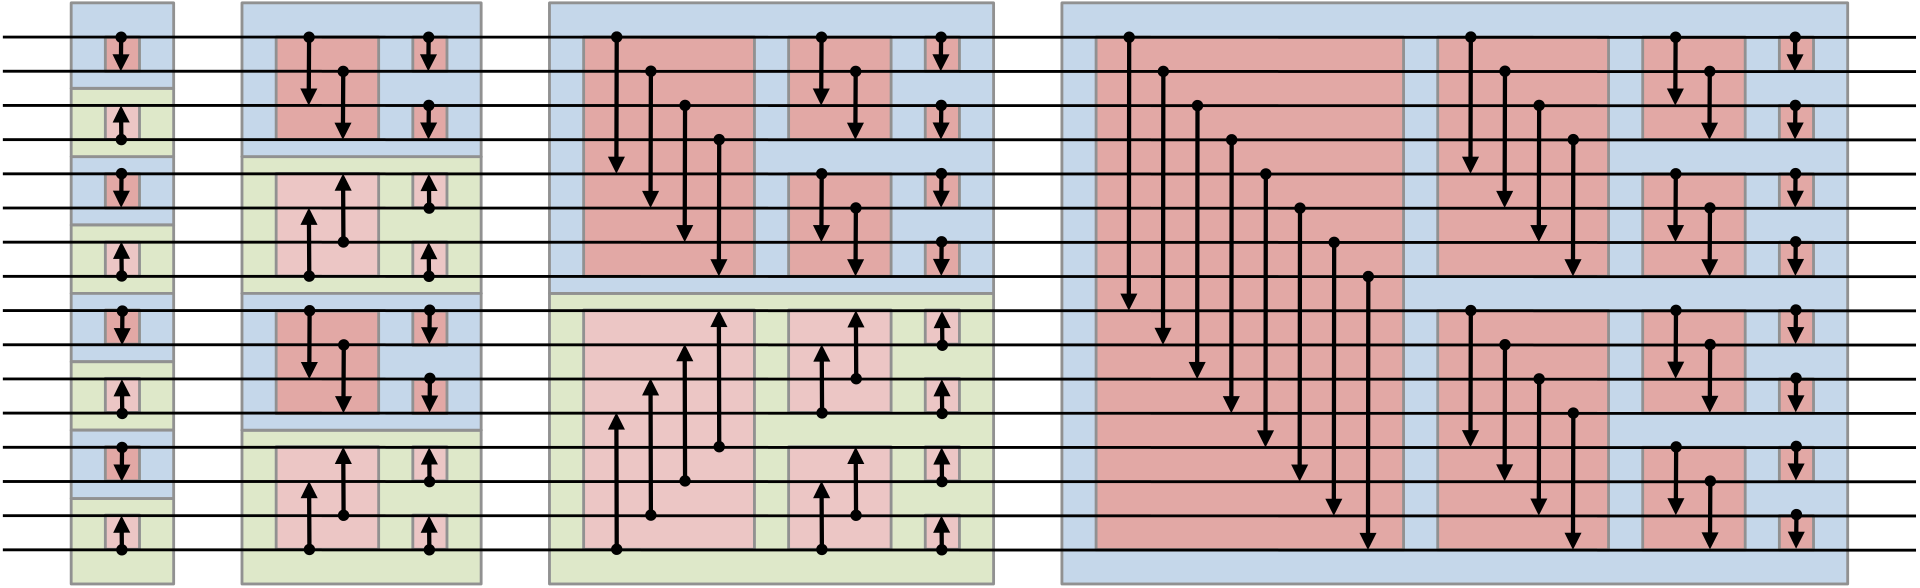
\includegraphics[width=0.8\linewidth]{bitonic-sort.png}

        \caption{\centering Битонная сортировка}

        \label{fig:bitonic-sort}

    \end{figure}

    Сразу бросается простота вычисления - глобальных шагов будет $\log(n)$. При этом каждый шаг содержит в себе аналог предыдущего. Синие прямоугольники - те, в которых элементы на следующем шаге будут идти по возрастанию. Зелёные - по убыванию. Стрелки показывают какой с каким элементы нужно менять. Если элемент у основания стрелки меньше того, на который она указывает, то их нужно поменять местами. Так достигается битонная последовательность. Сначала она не убывает, а потом не возрастает. На последнем шаге последовательность только возрастает. На первом - все элементы отсортированы в массиве только с собой.

    Алгоритмическая сложность сортировки - $O(n*\log(n))$

    \newpage

    \section{Практика}

    \subsection{Реализация сортировки пузырьком на CPU}

    \begin{lstlisting}[label=cpu-bubble-sort,caption=Сортировка пузырьком на CPU]
    long int sort(long int arr[]) {
        long int operations = 0;
        long int tmp = 0;

        for (long int i = 0; i < ARR_SIZE - 1; ++i) {
            for (long int j = 0; j < ARR_SIZE - 1; ++j) {
                if (arr[j] > arr[j + 1]) {
                    tmp = arr[j];
                    arr[j] = arr[j + 1];
                    arr[j + 1] = tmp;
                }
            }
        }

        return operations;
    }
    \end{lstlisting}

    \subsection{Реализация Quick-sort на CPU}

    \begin{lstlisting}[label=cpu-quick-sort,caption=Quicksort на CPU]
    long int sort(long int arr[], long int first, long int last)
    {
        long int operations = 0;
        long int i = first;
        long int j = last;
        long int pivot = last;
        long int tmp = 0;

        if (first < last) {
            while (i < j) {
                while (arr[i] <= arr[pivot] && i < last) {
                    i++;
                }
                while (arr[j] > arr[pivot]) {
                    j--;
                }
                if (i < j) {
                    tmp = arr[i];
                    arr[i] = arr[j];
                    arr[j] = tmp;
                }
            }
            tmp = arr[pivot];
            arr[pivot] = arr[j];
            arr[j] = tmp;
            operations += sort(arr, first, j - 1);
            operations += sort(arr, j + 1, last);
        }
        return operations;
    }
    \end{lstlisting}

    \subsection{Реализация параллельной сортировки пузырьком на GPU}

    \begin{lstlisting}[label=gpu-parallel-bubble-sort,caption=Параллельная пузырьковая сортировка на GPU]
    __global__ void sort (long int* data, unsigned long long* operations)
    {
        long int operationOnThread = ARR_SIZE / BLOCK_SIZE / 2 + 1;
        for (long int i = 0; i < ARR_SIZE / 2 + 1; ++i) {
            for (long int iOperation = 0; iOperation < operationOnThread; ++iOperation) {
                long int realIndex = (BLOCK_SIZE * iOperation + threadIdx.x) * 2;
                long int nextIndex = realIndex + 1;
                if (nextIndex < ARR_SIZE) {
                    if (data[realIndex] > data[nextIndex]) {
                        long int tmp = data[realIndex];
                        data[realIndex] = data[nextIndex];
                        data[nextIndex] = tmp;
                    }
                }
            }
            __syncthreads();
            for (long int iOperation = 0; iOperation < operationOnThread; ++iOperation) {
                long int realIndex = (BLOCK_SIZE * iOperation + threadIdx.x) * 2 + 1;
                long int nextIndex = realIndex + 1;
                if (nextIndex < ARR_SIZE) {
                    if (data[realIndex] > data[nextIndex]) {
                        long int tmp = data[realIndex];
                        data[realIndex] = data[nextIndex];
                        data[nextIndex] = tmp;
                    }
                }
            }
            __syncthreads();
        }
    }
    \end{lstlisting}

    \subsection{Реализация битонной сортировки на GPU}

    \begin{lstlisting}[label=gpu-bitonic-sort,caption=Битонная сортировка на GPU]
    __global__ void sort (long int* data, unsigned long long* operations)
    {
        long int arrSizeCopy = ARR_SIZE;
        int iterations = 0;
        while (arrSizeCopy > 0) {
            arrSizeCopy = arrSizeCopy >> 1;
            ++iterations;
        }
        long int fakeArrSize = 1 << iterations;
        int direction = 0;
        int half = 0;
        long int tmp = 0;

        for (int i = 0; i < iterations; ++i) {
            long int rectSize = 1 << (i + 1);
            long int halfRectSize = rectSize >> 1;

            long int stableRectSize = rectSize;
            while (rectSize > 1) {
                for (long int iElement = threadIdx.x; iElement < fakeArrSize; iElement += BLOCK_SIZE) {
                    // -1 - смотрит в начало, 1 - в конец
                    direction = -1;
                    if ((iElement / stableRectSize) % 2 == 0) {
                        direction = 1;
                    }

                    // 0 - половина большая к началу, 1 - к концу
                    half = 1;
                    if (iElement % rectSize < rectSize / 2) {
                        half = 0;
                    }
                    if ((direction == 1) && (half == 0)) {
                        if ((iElement < ARR_SIZE) && (iElement + halfRectSize < ARR_SIZE)) {
                            if (data[iElement] > data[iElement + halfRectSize]) {
                                tmp = data[iElement + halfRectSize];
                                data[iElement + halfRectSize] = data[iElement];
                                data[iElement] = tmp;
                            }
                        }
                    }
                    if ((direction == -1) && (half == 1)) {
                        if ((iElement < ARR_SIZE) && (iElement - halfRectSize < ARR_SIZE)) {
                            if (data[iElement] > data[iElement - halfRectSize]) {
                                tmp = data[iElement - halfRectSize];
                                data[iElement - halfRectSize] = data[iElement];
                                data[iElement] = tmp;
                            }
                        }
                    }
                }
                __syncthreads();
                rectSize = rectSize >> 1;
                halfRectSize = rectSize >> 1;
            }
        }
    }
    \end{lstlisting}


    \subsection{Дополнительно}

    Код из Листингов ~\ref{opcpu} и ~\ref{opgpu} был опущен из листингов выше. Потому что он много раз повторяется. Этот код компилируется только при выставлении макроса FULL. Из технологий CUDA здесь используется atomicAdd.

    В коде на CPU возвращается количество затраченных операций. В коде для GPU это количество передаётся по указателю.

    \begin{lstlisting}[label=opcpu,caption=Подсчёт количества операций в сортировках на CPU]
    #if defined(FULL)
        ++operations;
    #endif
    \end{lstlisting}

    \begin{lstlisting}[label=opgpu,caption=Подсчёт количества операций в сортировках на GPU]
    #if defined(FULL)
        atomicAdd(operations, (unsigned long long) 1);
    #endif
    \end{lstlisting}

    \subsection{Сравнение}

    Время замерялось от начала сортировки до конца сортировки встроенными средствами. То есть время на запуск и чтение уже опущено. Также подсчёт операций не влияет на скорость вычислений. В каждой программе объявлен макрос FULL, который влияет на компиляцию кусков кода с подсчётом. То есть столбцы заполнялись двумя независимыми запусками.

    Рассмитрим Таблицу ~\ref{table:comparsion1024}. На начальном этапе в 1024 элемента всё неплохо. У Quicksort большое преимущество по операциям, но уже здесь видно отставание от сортировок на GPU. В 15 раз.

    \begin{table}[h!]
        \centering
        \begin{tabular}{| l | r | l |}
            \hline
            {Название} & Операции (шт) & Время (с) \\
            \hline
            CPU пузырёк & 3.917.029 & 0.00251 \\
            \hline
            CPU quicksort & 724.128 & 0.00209 \\
            \hline
            GPU параллельный пузырёк & 8.951.704 & 0.00061 \\
            \hline
            GPU битонная & 2.473.857 & 0.00014 \\
            \hline
        \end{tabular}
        \caption{Сравнение для массива из 1024 элементов}
        \label{table:comparsion1024}
    \end{table}

    Рассмитрим Таблицу ~\ref{table:comparsion4096}. Стало интереснее - Quicksort почти догнал битонную сортировку по операциям. Больше по ним преимущества нет. Теперь разница между CPU и GPU стала более выражена. Видна выраженная разница между пузырьком и параллельным пузырьком. За счёт 1024 потоков время значительно уменьшилось.

    \begin{table}[h!]
        \centering
        \begin{tabular}{| l | r | l |}
            \hline
            {Название} & Операции (шт) & Время (с) \\
            \hline
            CPU пузырёк & 251.490.088 & 0,04554 \\
            \hline
            CPU quicksort & 11.682.064 & 0.03211 \\
            \hline
            GPU параллельный пузырёк & 102.992.488 & 0.00697 \\
            \hline
            GPU битонная & 13.266.457 & 0.00055 \\
            \hline
        \end{tabular}
        \caption{Сравнение для массива из 4096 элементов}
        \label{table:comparsion4096}
    \end{table}

    Рассмитрим Таблицу ~\ref{table:comparsion16384}. Предел разумного использования пузырька. Почти 1 секунда. При этом битонная сортировка догнала пузырёк из Таблицы ~\ref{table:comparsion1024}. Время почти такое же, элементов в 16 раз больше.

    \begin{table}[h!]
        \centering
        \begin{tabular}{| l | r | l |}
            \hline
            {Название} & Операции (шт) & Время (с) \\
            \hline
            CPU пузырёк & 1.006.372.810 & 0,84676 \\
            \hline
            CPU quicksort & 178.954.112 & 0.53797 \\
            \hline
            GPU параллельный пузырёк & 1.266.438.754 & 0.10325 \\
            \hline
            GPU битонная & 69.494.781 & 0.00249 \\
            \hline
        \end{tabular}
        \caption{Сравнение для массива из 16384 элементов}
        \label{table:comparsion16384}
    \end{table}

    Рассмитрим Таблицу ~\ref{table:comparsion65536}. Все сортировки кроме битонной перешагнули через 1 секунду. В остальном ничего интересного.

    \begin{table}[h!]
        \centering
        \begin{tabular}{| l | r | l |}
            \hline
            {Название} & Операции (шт) & Время (с) \\
            \hline
            CPU пузырёк & 16.110.614.796 & 15.40325 \\
            \hline
            CPU quicksort & 2.871.346.472 & 8.86929 \\
            \hline
            GPU параллельный пузырёк & 18.760.564.082 & 1.40010 \\
            \hline
            GPU битонная & 353.824.128 & 0.01258 \\
            \hline
        \end{tabular}
        \caption{Сравнение для массива из 65536 элементов}
        \label{table:comparsion65536}
    \end{table}

    Рассмитрим Таблицу ~\ref{table:comparsion131072}. Первый провал. Quicksort, основанный на рекурсии, не выдержал. Выдаёт ошибку на этих данных. Пузырёк после 60 миллиардов операций выдал результат, но потратил на это минуту. Дальше считать на CPU смысла нет.

    \begin{table}[h!]
        \centering
        \begin{tabular}{| l | r | l |}
            \hline
            {Название} & Операции (шт) & Время (с) \\
            \hline
            CPU пузырёк & 64.387.439.672 & 61.73878 \\
            \hline
            CPU quicksort & - & - \\
            \hline
            GPU параллельный пузырёк & 74.027.453.534 & 5.46474 \\
            \hline
            GPU битонная & 790.676.076 & 0.02783 \\
            \hline
        \end{tabular}
        \caption{Сравнение для массива из 131072 элементов}
        \label{table:comparsion131072}
    \end{table}

    Рассмитрим Таблицу ~\ref{table:comparsion524288}. Параллельный пузырёк тоже перестал иметь смысл. Полторы минуты. При этом битонная сортировка дошла до уровня параллельного пузырька на 16384 элемента. Пузырёк дошёл до ответа, но потратил на это больше 16 минут. Можно ещё заметит, что примерно одинаковое количетво операций на CPU и GPU выполнились в пузырьках с разницей во времени в 10 раз.

    \begin{table}[h!]
        \centering
        \begin{tabular}{| l | r | l |}
            \hline
            {Название} & Операции (шт) & Время (с) \\
            \hline
            CPU пузырёк & 1.030.784.790.368 & 992.33990 \\
            \hline
            CPU quicksort & - & - \\
            \hline
            GPU параллельный пузырёк & 1.172.264.597.452 & 91.28490 \\
            \hline
            GPU битонная & 3.883.140.794 & 0.128574 \\
            \hline
        \end{tabular}
        \caption{Сравнение для массива из 524288 элементов}
        \label{table:comparsion524288}
    \end{table}

    Дальнейшие эксперименты невозможны. Появлятся какое-то ограничение языка. Все 4 сортировки выдают ошибку.

    Дополнительно можно заметить, что Quicksort работает не сильно быстрее пузырька. Обычно всего в 2 раза. Скорее всего, это связано с оптимизациями со стороны компилятора.

    \newpage

    \section*{Заключение}

    Изучены алгоритмы сортировки, рассчитаные на параллельность. Реализованы 2 из них. Увиденно значительное преимущество больших вычислений на GPU перед CPU.

    \addcontentsline{toc}{section}{Заключение}

    Исходные коды всех программ, в том числе и программы для генерации последовательностей, можно найти по ссылке:

    \url{https://github.com/zalimannard/homework-4/tree/main/cuda}.


\end{document}
